\lecture{2}{vendredi 07 février 2020}
\vspace{-1.2cm}

\section{Introduction à la Traduction Automatique (TA)}

\epigraph{(…) the attempt to automate all, or part of the process\\ of translating from one human language to another.}{\textit{Arnold, 1993}}

Définition de Traduction Automatique: Automatisation du processus de traduction d'une $Phrase_{source} \rightarrow Phrase_{cible}$.
Il s'agit d'un domaine en constante évolution. Il envisage l'exercice de traduction comme s'il s'agissait d'un processus de décodage. \\

\noindent Il existe 3 types de traduction automatique:

\begin{enumerate}
    \item \textbf{Assimilation} Rompre la barrière des langues. Comprendre à minima le contenu d'un texte.
    On parle souvent de "gisting". Il y a de nombreuses applications: communication interne, blogs, journaux,
    sites web, documentation, littérature, etc. Il existe peu d'évaluation quantitative de ce genre de traduction.
    De toute façon, comment évaluer une telle traduction? Son but n'est pas d'être optimale, mais juste de couvrir
    au minimum la compréhension du texte source. Autre problème: de nombreux services de traduction online stockent
    les textes source, il y a donc un risque de problèmes de protection des données.
    \item \textbf{Communication} TA pour la communication orale (interprétation). Deux technologies centrales: la synthèse vocale et la TA.
    \item \textbf{Dissémination} TA du traducteur. Son but est de publier un texte dans une autre langue.
    La qualité doit être égale à la TH (traduction humaine), et il y a deux conditions pour que ce soit le cas
    \begin{enumerate}
        \item \textbf{Domaine limité} On essaye d'avoir une TEAHQ (Traduction Entièrement Automatique et de Haute Qualité) / FAHQT (Fully Automatic High Quality Translation).
        Ceci est impossible si on essaye de traduire dans un scope de langage énorme.
        Donc on essaye de focaliser les efforts sur un sous-langage (e.g. un traducteur spécialisé dans le domaine de la météo).
        \item \textbf{Intervention humaine} Un humain (traducteur ou réviseur) intervient dans le processus de traduction,
        de deux façons possibles: pré-édition (simplification du texte, éviter les phrases longues et les longs groupes nominaux, etc)
        et post-édition (PE). De nouveaux métiers se créent (sujet complexe car on dit également que d'autres métiers se perdent).
    \end{enumerate}
\end{enumerate}

\noindent Dans les prochains chapitres on analysera les trois types de systèmes de traduction automatique:

\begin{enumerate}
    \item \textbf{Systèmes linguistiques} Rule-based machine translation (RBMT) \footnote{\hyperref[sec:RBMT]{Chapitre 3}}
    \item \textbf{Systèmes fondés sur les corpus (data-driven)} \footnote{\hyperref[sec:corpus]{Chapitre 4}}
    \begin{enumerate}
        \item Statistical machine translation (SMT)
        \item Neuronal machine translation (NMT) \\
    \end{enumerate}
\end{enumerate}

\noindent\textbf{Post-édition VS Traduction Humaine}
\begin{enumerate}
    \item Rentable, 20\% à 40\% de gain de productivité selon les études (e.g. Plitt \& Masselot 2010, Green 2013)
    \item Ne conduit pas nécessairement à plus d'erreurs ou des textes de moins bonne qualité
    \item "Posteditese" (e.g. Toral 2019, Kubler 2019) (TODO: Add definition here)
\end{enumerate}

\noindent\textbf{Nouvelles applications de la TA\\}

\begin{minipage}[t]{0.5\textwidth}
\begin{itemize}
\item Sous-titrage
\item TA d'images
\item TA vers des langues simplifiées \\(e.g. Simple Wikipedia)\\
\end{itemize}
\end{minipage}
\begin{minipage}[t]{0.5\textwidth}
\begin{itemize}
\item TA vers des pictogrammes
\item TA vers la langue des signes
\end{itemize}
\end{minipage}

\noindent\textbf{Problèmes posés par la TA}

\begin{enumerate}
    \item \textbf{Ambigüité}
    \begin{enumerate}
        \item Lexicale
        \item Structurale
    \end{enumerate}
    \item \textbf{Divergences}
    \begin{enumerate}
        \item Lexicales (décalages)
        \item Structurales
    \end{enumerate}
    \item \textbf{De nombreuses traductions possibles}
        Comment choisir la meilleure (ou la seule correcte)?
\end{enumerate}

\noindent\textbf{Divergences structurales\\}

(TODO)

- Typologiques
    - Ordre des mots (e.g. SVO en FR, SOV en Japonais et VSO en Arabe)
    - Pronoms
- Idiosyncratiques (propres à une langue)
- Générales à la syntaxe d'une langue
- Déclenchées par un mot particulier

Du plus facile au plus compliqué à résoudre (Vandooren 1993)
- Catégorielle (e.g. nom vers adjectif)
- Syntagmatique
- Lexicale
- De densité lexicale
- Thématique
- Prédicative

Statistiques des divergences (Dorr 2002)
- Part of Speech (98\%)
- Phrase/Light verb (83\%)
- Structural (35\%)
- Heads swap (8\%)
- Arguments swap (6\%)

(END OF TODO)

\newpage

\section{Les systèmes linguistiques (RBMT)}
\label{sec:RBMT}

Les premiers systèmes de TA commerciaux et sur internet (BabelFish, Altavista, etc).
Ils étaient les seuls à être développés jusqu'en 2006 (avant l'apparition de SMT et NMT, voir chapitre suivant).

À l'époque ils étaient les seuls à faire de la TEAHQ (à mettre en perspective, la qualité n'est plus considérée aussi bonne quand on la compare aux résultats actuels).

Beaucoup de différences entre ces systèmes, mais quelques points communs:

\begin{enumerate}
    \item \textbf{Analyse linguistique} pour extraire le sens de la phrase
    ("natural language understanding")
    \begin{enumerate}
        \item Pipeline linguistique (on passe par différents niveaux: lexical,
        syntaxique, sémantique, pragmatique/extralinguistique)
    \end{enumerate}
    \item \textbf{Transfert}
    \item \textbf{Géneration} de la langue cible
\end{enumerate}

\subsection{Systèmes directs/minimalistes}

Les plus simples. Fonctionnent en deux étapes:

\begin{enumerate}
    \item \textbf{Compréhension minimale (lexicale)}
    \begin{enumerate}
        \item Segmentation en mots
        \item Tagging de catégorie grammaticale de chaque mot
    \end{enumerate}
    \item \textbf{Traduction} mot à mot avec un dictionnaire bilingue
\end{enumerate}

\textbf{Dictionnaire}

La ressource principale des systèmes directs (pas de grammaires).

Il contient toutes les informations nécessaires pour la compréhension et la traduction,
c'est à dire au minimum: le mot/expression source/cible, les informations lexicales monolingues sur le mot/expression source/cible et les informations bilingues.\\

\textbf{Informations bilingues}

\begin{enumerate}
    \item Traduction mots/expressions
    \item Tests (transfer conditions)
    \begin{itemize}
        \item Permettent de choisir la bonne traduction s'il y en a plusieurs.
        \item Devraient porter sur tous les niveaux linguistiques (lexical, synt, sem et pragmatique).
        \item e.g. : grow (élever, cultiver ou grandir?)
    \end{itemize}
    \item Actions
\end{enumerate}

\textbf{Types de tests}

\begin{itemize}
    \item Test sur les informations morphologiques (e.g. singulier vs pluriel)
    \item Test sur la syntaxe (rection) (e.g. traduction d'un verbe dépendant de
    l'objet auquel il s'applique)
    \item Test sur le type sémantique (sens) (e.g. traduction d'un verbe dépendant
    du type de sujet, humain ou animal)
    \item Test sur le domaine (e.g. le mot "bug" en informatique ou en biologie)
    \item Test sur les propriétés encyclopédiques (ontologie) (e.g. traductions
    entières de bouts de phrases stockées)\\
\end{itemize}

Dans les systèmes directs, les tests portent uniquement sur le niveau lexical:
nombre, genre, mots dans contexte.

Exemple: SystranNet (2018)

to grow (context: child, etc.) = grandir

to grow (context: chicken, etc.) = élever

to grow (context: corn, salad, etc.) = cultiver \\

\textbf{Actions}

Permettent de traiter les divergences, c'est-à-dire de changer la syntaxe sous
certaines conditions.

(TODO)
---
en TROIS étapes??

Compréhension
    Problèmes:
        - Analyse morphologique et résolution des homographes ca
Traduction
    Problèmes:
        - Tests/actions limités
        - 1 dictionnaire par paire de langues
Génération
    Problèmes:
        - Architecture de type "transformateur"
        - Pas de connaissances grammaticales de la langue cible, comme dans les systèmes indirects

---
Ne peut donner des résultats exploitables que si sous-langage et dictionnaire bien spécialisé

(END TODO)

\subsection{Systèmes indirects/maximalistes}

Tandis que les systèmes directs focalisaient le moins possible sur le niveau de
la compréhension (minimalistes), les systèmes indirects eux le font au plus possible.

Ils sont les seuls systèmes linguistiques à faire de la TEAHQ.\\

\textbf{Caractéristiques}

\begin{enumerate}
    \item Ne restent pas au niveau lexical. Font au moins une analyse syntaxique complète, avec une grammaire, et représentent ainsi le sens de la phrase à traduire
    \item Ne mettent pas en relation directe des mots, mais mettent en correspondance des représentations
\end{enumerate}

\textbf{Avantages}

\begin{enumerate}
    \item Représentent l’ambigüité structurale
    \item Évitent les erreurs de désambigüisation lexicale
\end{enumerate}

Systèmes de TA indirects
    - Par transfert
    - Par interlangue

Théories de la traduction circa '90
    - Deverbalisation du sens
    - Production

\vspace{1cm}

\textbf{Triangle de Vauquois}

\resizebox{0.85\textwidth}{!}{
    

\tikzset{every picture/.style={line width=0.75pt}} %set default line width to 0.75pt

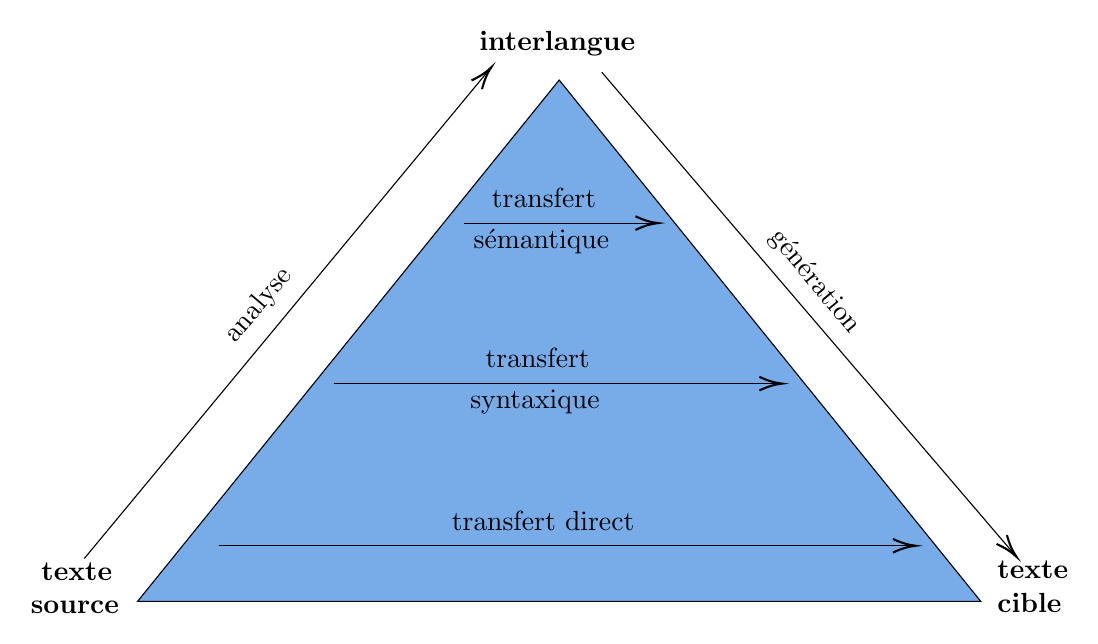
\begin{tikzpicture}[x=0.75pt,y=0.75pt,yscale=-1,xscale=1]
%uncomment if require: \path (0,777); %set diagram left start at 0, and has height of 777

%Shape: Triangle [id:dp37993567465978106]
\draw  [fill={rgb, 255:red, 74; green, 144; blue, 226 }  ,fill opacity=0.75 ] (297.6,38.51) -- (500.73,289.68) -- (94.48,289.68) -- cycle ;
%Straight Lines [id:da3821484196531547]
\draw    (133.92,262.88) -- (467.33,262.88) ;
\draw [shift={(469.33,262.88)}, rotate = 180] [color={rgb, 255:red, 0; green, 0; blue, 0 }  ][line width=0.75]    (10.93,-3.29) .. controls (6.95,-1.4) and (3.31,-0.3) .. (0,0) .. controls (3.31,0.3) and (6.95,1.4) .. (10.93,3.29)   ;
%Straight Lines [id:da35117354484946606]
\draw    (189.05,184.77) -- (403.01,184.77) ;
\draw [shift={(405.01,184.77)}, rotate = 180] [color={rgb, 255:red, 0; green, 0; blue, 0 }  ][line width=0.75]    (10.93,-3.29) .. controls (6.95,-1.4) and (3.31,-0.3) .. (0,0) .. controls (3.31,0.3) and (6.95,1.4) .. (10.93,3.29)   ;
%Straight Lines [id:da19792780780087094]
\draw    (251.85,107.43) -- (343.28,107.43) ;
\draw [shift={(345.28,107.43)}, rotate = 180] [color={rgb, 255:red, 0; green, 0; blue, 0 }  ][line width=0.75]    (10.93,-3.29) .. controls (6.95,-1.4) and (3.31,-0.3) .. (0,0) .. controls (3.31,0.3) and (6.95,1.4) .. (10.93,3.29)   ;
%Straight Lines [id:da14845116336104136]
\draw    (68.83,269.01) -- (263.59,33.92) ;
\draw [shift={(264.87,32.38)}, rotate = 489.64] [color={rgb, 255:red, 0; green, 0; blue, 0 }  ][line width=0.75]    (10.93,-3.29) .. controls (6.95,-1.4) and (3.31,-0.3) .. (0,0) .. controls (3.31,0.3) and (6.95,1.4) .. (10.93,3.29)   ;
%Straight Lines [id:da355143642126483]
\draw    (318.12,34.73) -- (516.63,266.67) ;
\draw [shift={(517.93,268.19)}, rotate = 229.44] [color={rgb, 255:red, 0; green, 0; blue, 0 }  ][line width=0.75]    (10.93,-3.29) .. controls (6.95,-1.4) and (3.31,-0.3) .. (0,0) .. controls (3.31,0.3) and (6.95,1.4) .. (10.93,3.29)   ;

% Text Node
\draw (257.83,13.54) node [anchor=north west][inner sep=0.75pt]   [align=left] {\textbf{{interlangue}}};
% Text Node
\draw (507.5,269.15) node [anchor=north west][inner sep=0.75pt]   [align=left] {\textbf{texte}\\\textbf{cible}};
% Text Node
\draw (41.79,269.92) node [anchor=north west][inner sep=0.75pt]   [align=left] {\textbf{ texte}\\\textbf{source}};
% Text Node
\draw (244.58,244.81) node [anchor=north west][inner sep=0.75pt]   [align=left] {transfert direct};
% Text Node
\draw (260.87,166.7) node [anchor=north west][inner sep=0.75pt]   [align=left] {transfert};
% Text Node
\draw (253.52,186.61) node [anchor=north west][inner sep=0.75pt]   [align=left] {syntaxique};
% Text Node
\draw (263.94,89.35) node [anchor=north west][inner sep=0.75pt]   [align=left] {transfert};
% Text Node
\draw (255.12,109.26) node [anchor=north west][inner sep=0.75pt]   [align=left] {sémantique};
% Text Node
\draw (132.51,159.58) node [anchor=north west][inner sep=0.75pt]  [rotate=-310.5] [align=left] {analyse};
% Text Node
\draw (406.04,106.74) node [anchor=north west][inner sep=0.75pt]  [rotate=-50.3] [align=left] {génération};


\end{tikzpicture}

}

\vspace{1cm}

Axe vertical: profondeur d'analyse, niveau d'analyse syntaxique
    e.g. directs on reste au niveau lexical, transfert au moins syntaxique, interlingue on va jusqu'au niveau sémantique

Axe horizontal: quantité de connaissance contrastive qu'il faut pour passer d'une langue à l'autre

Systèmes par transfert:

    - Module d'analyse: syntaxique et spécifique à la langue (par définition)
    - Module de transfert: règles de transfert
    - Génération: Représentation syntaxique cible -> texte cible

Types de règles de transfert:

    - Lexicales: équivalences entre les mots
    - Structurales: liens entre les éléments structuraux (e.g. verb --> verbe, subject -> sujet)
    - Semi-lexicales: permettent de changer la syntaxe de la phrase via des tests et actions

Avantages:

Systèmes par interlangue

Problèmes:
    - Concepts: définir l'ensemble des concepts et choisir le bon contexte. Ceci oblige à faire des distinctions qui ne sont pas nécessaires pour toutes les paires de langues. E.g. espagnol: différence entre le mot pour poisson vivant et poisson mort.
    - Granularité de la représentation:

Dionysus:
    Facteurs pragmatiques:
        Formalité: formel ou pas
        Simplicité: simple ou pas
        Force
        Couleur
        Respect
    Relations entre les phrases
        Domaine (cause, motivation), textuelle (conclusion, reformulation), temporelle
    Attitude
        emphase, croyance, négative, positive
    Intention
        question, requête


Différences transfert vs interlangue
    Types de représentation
        Transfert: spécifique à la langue
    Connaissances contrastives
    Type de traduction
        Transfert: littérale, on préserve la syntaxe
        Interlangue: par paraphrase, on va vers le sens et on génère avec le sens de la phrase

Exemples:
    Première par transfert
    Deuxième par interlangue

Exemples d'interlangue:
    UNL (ONU)
    Ontologie -> concepts communs à toutes les langues

    Esperanto
    Distributed Language Translation


Contexte positif pour l'interlangue
    - Sous dommaine, si possible technique
        - Travail humain énorme
    - Contexte multilingue
        - un seul système, au lieu d'un système par chaque paire de langues
    - Langues très différentes
        - e.g. Japonais, le transfert ne fonctionne pas vu la différence énorme au niveau de la grammaire

Systèmes linguistiques résumé
    Très ambitieux
    Hypothèses:
        - Bcp de régularités entre les langues: faux
        - Peu d'exceptions: faux
        - Règles peuvent être définies par des experts
    Problèmes:
        - Robustesse: les langues ne sont pas si régulières
        - Chers et lents à développer
        - Statiques: figés dans le temps, n'apprennent pas via de nouveaux corpus.
